\documentclass[11pt]{article}
% ============================================================================
%  Conversational Search Token-Cost Optimization: Savings Forecast
%  and the Case for TIP as a Cost-Optimization Platform
%  Internal technical report - DRAFT (assumptions flagged; calibrate vs telemetry)
% ============================================================================
\usepackage[a4paper,margin=1in]{geometry}
\usepackage[T1]{fontenc}
\usepackage{lmodern}
\usepackage{microtype}
\usepackage{amsmath,amssymb}
\usepackage{booktabs}
\usepackage{tabularx}
\usepackage{graphicx}
\usepackage{xcolor}
\usepackage{enumitem}
\usepackage{caption}
\usepackage[hidelinks]{hyperref}
\definecolor{linkc}{HTML}{6D28D9}
\hypersetup{colorlinks=true, linkcolor=linkc, citecolor=linkc, urlcolor=linkc}
\newcommand{\code}[1]{\texttt{\small #1}}
\graphicspath{{../scripts/forecast/results/figures/}{../scripts/eval/results/figures/}}

\title{\textbf{Conversational-Search Token-Cost Optimization:\\
A Savings Forecast and the Case for TIP as a Cost Platform}}
\author{Sean Poyner \\ \small Use Case Engineering, Marriott D\&AI}
\date{June 2026 \quad\small(DRAFT - assumptions flagged for calibration)}

\begin{document}
\maketitle

\begin{abstract}
Marriott's guest-facing AI conversational search (the \code{mi-conversational-ai-agent} /
``Ask Bonvoy'' NLS experience) runs on \textbf{Gemini 3.1 Flash-Lite via the TIP.ai LiteLLM
proxy} (Jira GENAI-1412, WEB-194505) and is under active cost review (the Cost Optimization
Alignment workstream). This report forecasts how far its token cost can be cut \emph{at fixed
answer quality}. Under an explicit, parameterized model (calibrate against Adobe event206-208
and Dynatrace token telemetry), the monthly run-rate baseline is on the order of
\textbf{\$540K/month} at current assumptions, of which an \textbf{expected $\sim$75\%} is
recoverable. The three levers, in order of impact: (1) \textbf{caching} the large fixed prefix
re-sent every turn ($\sim$35\% alone, 22--42\% across a hit-rate sweep, zero quality risk);
(2) \textbf{context/RAG pruning} + history compaction ($\sim$57\% combined); and (3) a
\textbf{default model swap to \code{gemma4:31b} on Vertex} - a \emph{managed, in-GCP} model that
is $\sim$42\% cheaper than Flash-Lite at this token mix and, in our head-to-head measurement, of
\emph{statistically on-par} quality ($\sim$75\% combined, up to 87\% aggressive). The incumbent
Flash-Lite is \emph{not} Google's cheapest competent tier, so model selection is a real lever
here; by contrast, \emph{self-hosting} the same model on Amazon is $\sim$26$\times$ more
expensive per token and is a data-residency/control play, not a cost lever. We recommend a
prescriptive sequence (caching $\rightarrow$ pruning $\rightarrow$ \code{gemma4:31b}-on-Vertex
default), gated by a strict do-no-harm quality eval, delivered as a reusable \textbf{TIP SDK
platform capability} (router + caching + context-pruning middleware) emitting spend metrics to
the control plane.
\end{abstract}

\section*{Executive summary}
\begin{itemize}[leftmargin=1.3em,itemsep=2pt]
\item \textbf{Confirmed setup:} Gemini 3.1 Flash-Lite (\$0.25 in / \$1.50 out per 1M) via the
TIP.ai LiteLLM proxy (GENAI-1412, WEB-194505). Optimization middleware lands exactly where
traffic already flows.
\item \textbf{Baseline (assumption-driven):} $\sim$24M conversations/month $\rightarrow$
$\sim$1.9T input tokens/month $\rightarrow$ \textbf{$\sim$\$540K/month} ($\sim$\$0.022/conversation).
Input is $\sim$98\% of tokens and scales \emph{quadratically} with conversation length, because
the 15k+ system prompt and RAG are re-sent every turn and history grows.
\item \textbf{Lever 1 - caching (no quality risk):} 35\% (expected); 22--42\% across a 50--95\%
hit-rate sweep.
\item \textbf{Lever 2 - context/RAG pruning:} $\rightarrow$ $\sim$57\% combined.
\item \textbf{Lever 3 - swap default to \code{gemma4:31b} on Vertex:} managed, in-GCP,
$\sim$42\% cheaper than Flash-Lite at \emph{measured on-par} quality $\rightarrow$ \textbf{$\sim$75\%
combined (expected), up to 87\% aggressive}.
\item \textbf{Self-host on Amazon is NOT a cost lever:} the same model self-hosted is
$\sim$\$4/1M (owned-compute est) vs \code{gemma4:31b}-on-Vertex's $\sim$\$0.16/1M; justify it on
data residency/control, not unit cost.
\item \textbf{Recommendation:} caching first, then pruning, then the \code{gemma4:31b}-on-Vertex
default behind a strict quality gate; build it once as a TIP SDK platform capability feeding the
control plane.
\end{itemize}
Three audiences: a Gen-AI exec cost view (\S\ref{sec:forecast}), a search-team lever playbook
(\S\ref{sec:levers}, \S\ref{sec:quality}), and a TIP platform case (\S\ref{sec:platform}).

\section{Context and scope}
Guest-facing conversational search (DDC events 206-208; the AI-for-Search workstream; products
\code{mi-conversational-ai-agent}/``Ask Bonvoy''/NLS/Polaris) runs on GCP and, per Jira, on
\textbf{Gemini 3.1 Flash-Lite through the TIP.ai LiteLLM proxy}. Token costs are capitalizable
and under exec attention (Paul Dyrwal). Sean has built a LiteLLM model router for the TIP SDK
(delivery imminent), and Kenny Hammerlund's control plane tracks per-agent spend with
conversational search as its first use case. Objective (from alignment): a \emph{max-defensible
savings curve} at fixed quality, with the do-no-harm constraint (no regression to
Step-Conversion-to-RLM or Visitor-Conversion) treated as sacred.

\section{Method}
A single parameterized model (\code{scripts/forecast/conv\_search\_forecast.py}); every input is
explicit and auditable, to be calibrated against Adobe event206-208 volume, Dynatrace token
telemetry, and the Egor/Kenny cost baseline. Model price/quality options reuse the LiteForge
cross-provider cost-quality study (25 models, graded benchmarks, bootstrap CIs). Rigor:
conservative/expected/aggressive \textbf{bands}, a \textbf{sensitivity} (tornado) analysis, and
bootstrap CIs where inputs are measured (model quality). Horizon: monthly run-rate.

\paragraph{Why input scales quadratically.} For a conversation of $T$ turns with fixed system
$S$, RAG $R$, per-turn query $q$ and output $o$, total input tokens are
\[
\text{input} = T\,(S+R+q) + (q+o)\,\frac{T(T-1)}{2},
\]
because $S$ and $R$ are re-sent every turn and history accumulates. The first term is what
caching attacks; the second is what history compaction attacks.

\section{Baseline forecast}
\label{sec:forecast}
At current assumptions (270M Bonvoy members $\times$ 3\% adoption $\times$ 3 conversations/mo
$\times$ 4 turns; system 15k, RAG 4k, output 400 tokens; Gemini 3.1 Flash-Lite at
\$0.25/\$1.50 per 1M): $\sim$24.3M conversations/month, $\sim$1.91T input + 38.9B output
tokens/month, \textbf{$\sim$\$540K/month}, \$0.022/conversation. The baseline is most sensitive
to conversations-per-user, adoption, and input price (Figure~\ref{fig:tornado}); the 3\%
adoption figure scales the whole result linearly and should be validated against Adobe first.

\section{The savings levers}
\label{sec:levers}
Figure~\ref{fig:curve} shows cumulative savings as the levers are applied in order.

\begin{figure}[h]
\centering
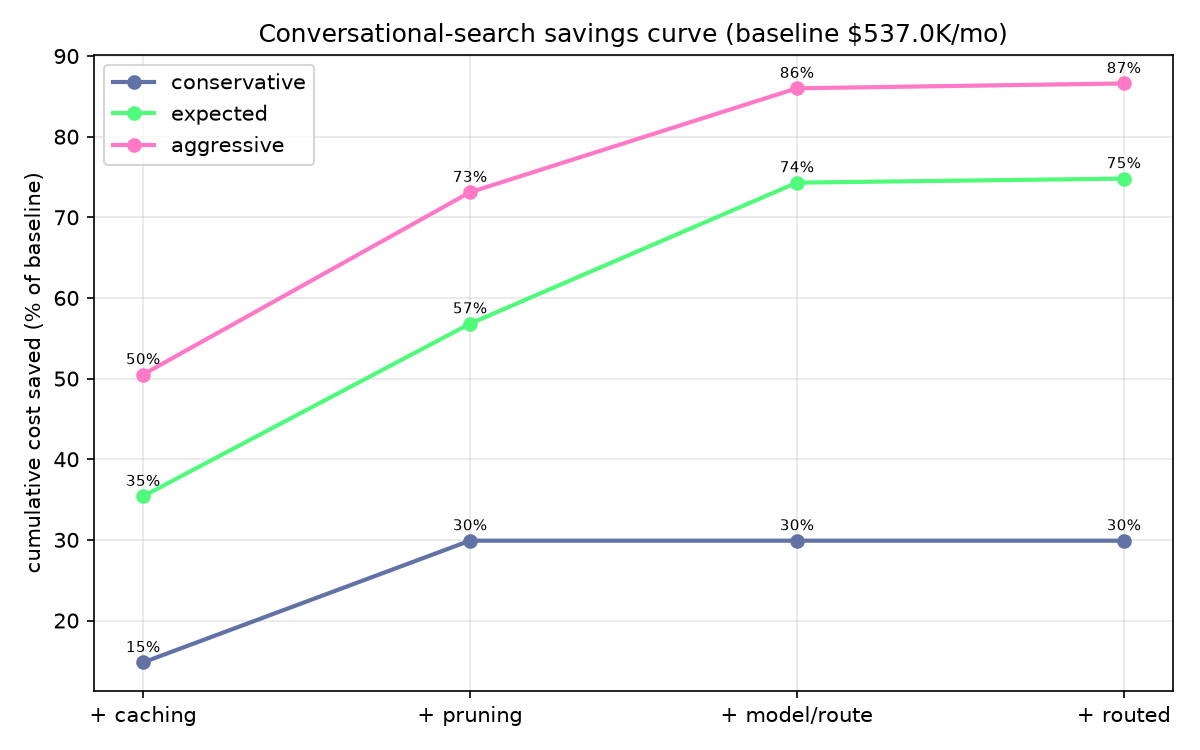
\includegraphics[width=0.80\textwidth]{savings_curve.png}
\caption{Cumulative cost saved vs baseline as levers stack, for three scenarios. Caching and
pruning carry the first $\sim$57\%; the \code{gemma4:31b}-on-Vertex default swap adds $\sim$18
more points (expected).}
\label{fig:curve}
\end{figure}

\paragraph{(1) Caching - the safest win.} The 15k+ system prompt plus the stable share of RAG
is a fixed prefix re-sent every turn; caching it (Vertex context caching) bills those tokens at
a fraction of input price on a hit. Figure~\ref{fig:cache}: \textbf{22\% saved at a 50\% hit
rate, rising to 42\% at 95\%}. Ship this first - no model change, no quality risk. (Open item:
confirm Vertex/TIP caching support and the cached-token discount.)

\begin{figure}[h]
\centering
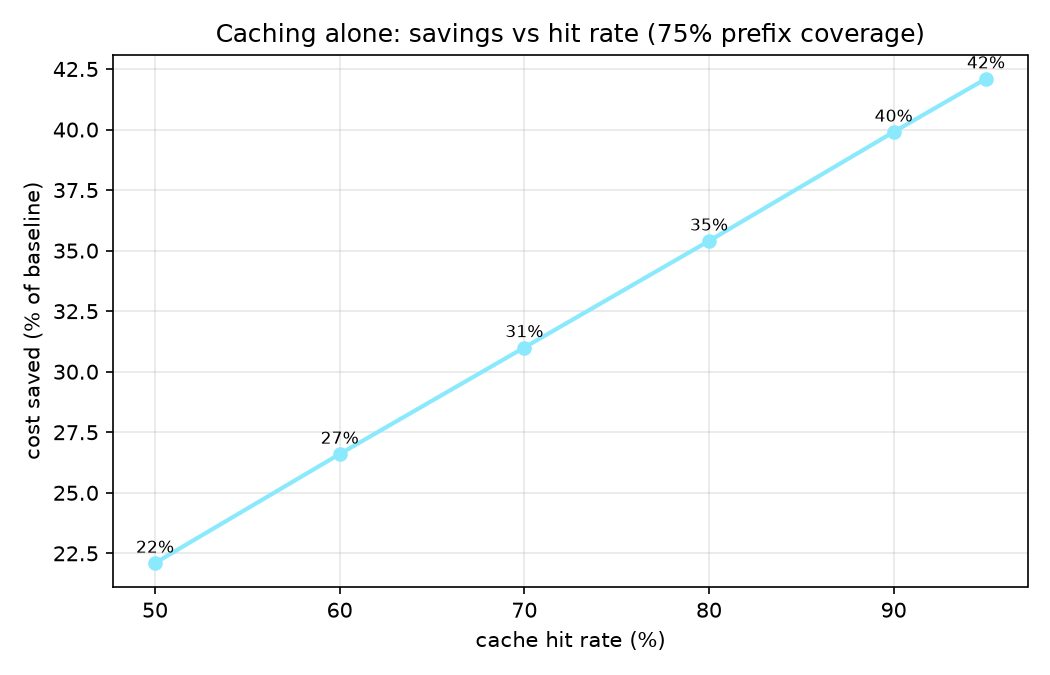
\includegraphics[width=0.70\textwidth]{cache_sweep.png}
\caption{Caching alone: cost saved vs cache hit rate at 75\% prefix coverage.}
\label{fig:cache}
\end{figure}

\paragraph{(2) Context + RAG pruning, history compaction.} Trimming the system prompt,
tightening retrieval, and compacting/windowing history attack the variable cost (and the
quadratic history term). With caching this reaches $\sim$57\% (expected).

\paragraph{(3) Swap the default to \code{gemma4:31b} on Vertex.} The incumbent Gemini 3.1
Flash-Lite (\$0.25/\$1.50) is \emph{not} Google's cheapest competent tier. Managed, per-token
\textbf{\code{gemma4:31b} on Vertex} (published \$0.15/\$0.60) is $\sim$42\% cheaper at this
input-heavy mix (Figure~\ref{fig:bvb}). Crucially, this is not a quality trade: in a
head-to-head on the same 290 graded prompts, \code{gemma4:31b} scored \textbf{0.866 vs
Flash-Lite's 0.859} (paired difference $+0.007$, 95\% CI $[-0.017, +0.031]$) - \emph{statistically
on par}, tied per-benchmark with a slight edge on GSM8K and MBPP. Because quality is non-inferior,
this is a \textbf{default swap for $\sim$all traffic}, not just an easy-tail route, taking expected
savings from $\sim$57\% to $\sim$75\%. (A hard tail can still escalate to Flash-Lite/Gemini Pro
for safety, via an escalate-on-failure cascade gated by the grounding check rather than an
up-front difficulty predictor; see Section~\ref{sec:hardtail}.) A learned router adds little over
this static swap at near-parity (the LiteForge finding), so we credit selection, not routing
cleverness.

\paragraph{(4) Self-host on Amazon - residency, not cost.} The same model self-hosted on Amazon
(Bedrock/EKS, owned-compute estimate) is $\sim$\$4/1M - roughly $\sim$26$\times$ the managed
\code{gemma4:31b}-on-Vertex price and $\sim$15$\times$ Flash-Lite (Figure~\ref{fig:bvb}).
Self-host only approaches parity at very high utilization; its value here is data
residency/control or custom fine-tuning, argued on those terms.

\begin{figure}[h]
\centering
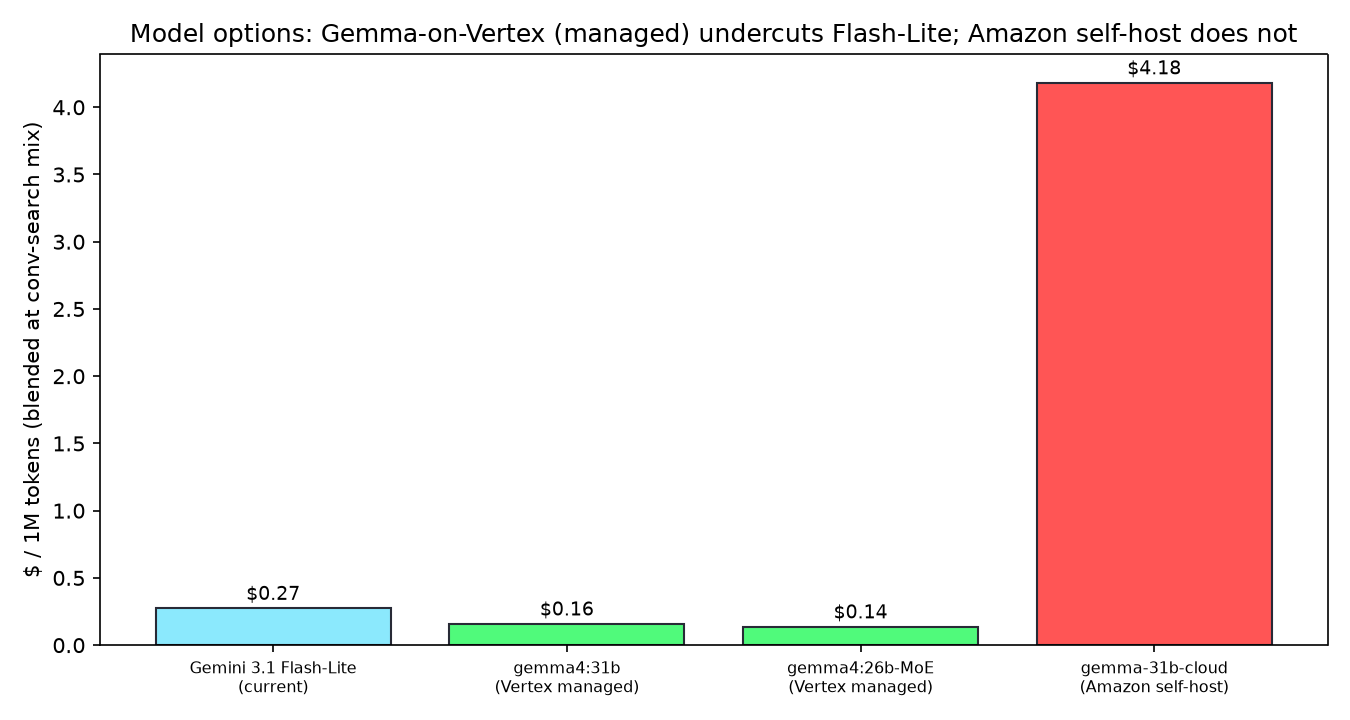
\includegraphics[width=0.92\textwidth]{build_vs_buy.png}
\caption{Blended \$/1M at the conversational-search token mix. Managed \code{gemma4:31b}-on-Vertex
undercuts the incumbent Flash-Lite at on-par quality; Amazon self-host does not (residency
option).}
\label{fig:bvb}
\end{figure}

\begin{figure}[h]
\centering
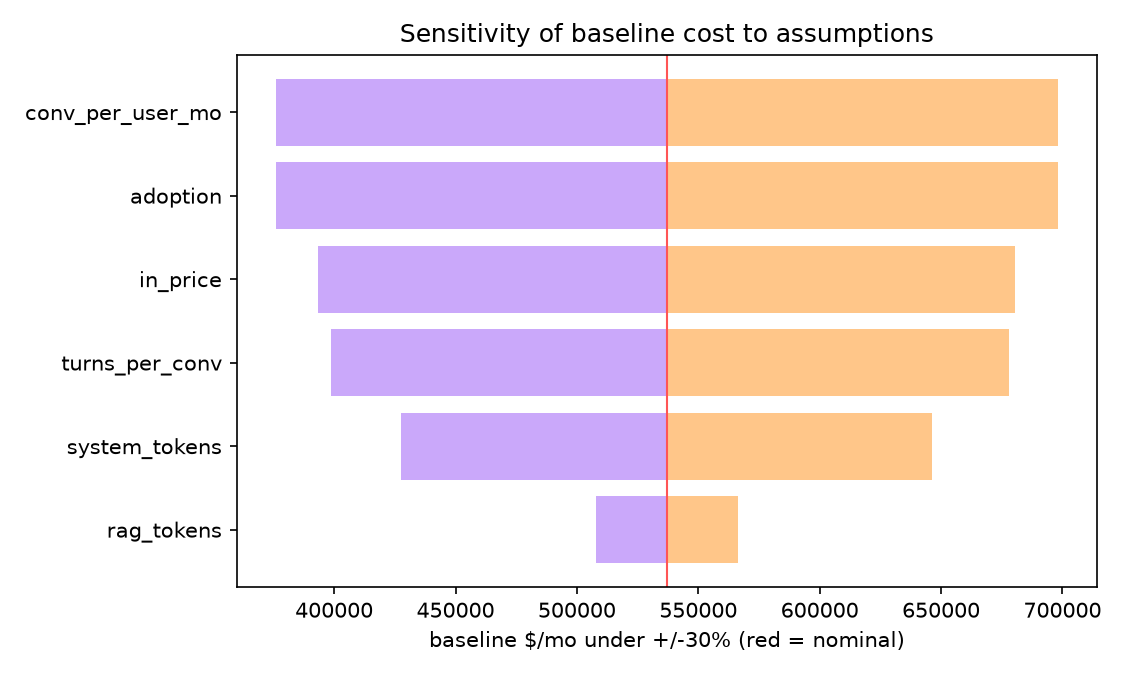
\includegraphics[width=0.70\textwidth]{tornado.png}
\caption{Sensitivity of the monthly baseline to each assumption ($\pm$30\%). Volume
(conversations/user, adoption) and price dominate; validate these first.}
\label{fig:tornado}
\end{figure}

\section{Quality gate (do-no-harm)}
\label{sec:quality}
No change ships unless it is \emph{strictly non-inferior} to the Gemini-3.1-Flash-Lite baseline.
The \code{gemma4:31b} swap already clears this on public benchmarks (paired diff $+0.007$, CI
$[-0.017,+0.031]$ above); the production gate repeats the same test on \textbf{real
conversational-search queries} using the LiteForge evaluation harness with Lakshmi Nimmagadda's
existing eval set, scoring each candidate by an LLM judge \emph{and} a grounding/faithfulness
check (guest answers must be supported by retrieved inventory/policy - no hallucinated rates),
with bootstrap CIs. Recommended rollout: shadow $\rightarrow$ gated A/B with auto-rollback on KPI
regression; execution detail left to the search team.

\section{Recommendation}
\textbf{Primary sequence (prescriptive):}
\begin{enumerate}[leftmargin=1.5em,itemsep=1pt]
\item \textbf{Enable prefix caching} (system prompt + static RAG). Biggest safe win
(22--42\% alone). Confirm Vertex/TIP caching support first.
\item \textbf{Prune context} (trim system prompt, tighten retrieval, compact history)
$\rightarrow$ $\sim$57\% combined.
\item \textbf{Swap the default to \code{gemma4:31b}-on-Vertex} (managed, in-GCP) behind the
quality gate $\rightarrow$ $\sim$75\% combined.
\end{enumerate}
\textbf{Options on the curve:} the conservative/expected/aggressive band ($\sim$30\% / $\sim$75\%
/ $\sim$87\%) lets leadership pick an operating point against effort and risk. \textbf{Self-host
on Amazon} only if data-residency/control or fine-tuning requires it - not a unit-cost win.
(Capitalization note: dev-phase token costs are capitalizable; finance to confirm treatment.)

\section{TIP as a cost-optimization platform}
\label{sec:platform}
These levers should be built once, in the TIP SDK, as a reusable platform capability: the
already-announced LiteLLM \textbf{router} plus \textbf{caching} and \textbf{context-pruning}
middleware, emitting \textbf{spend metrics} to Kenny's control plane (which both visualizes
spend and governs the routing/guardrail config). Conversational search already calls the TIP
LiteLLM proxy (WEB-194505), so it is the first and highest-volume tenant; the same capability
then serves ConEng consumers and other agents. This analysis forecasts the savings; the router
policy itself is already designed. One refinement from the routing studies below: the hard-tail
mechanism should be an \emph{escalate-on-failure cascade}, not an up-front difficulty predictor.

\section{Routing the hard tail: evidence from routing studies}
\label{sec:hardtail}
Lever 3 makes \code{gemma4:31b} the default; a small fraction of hard queries may still need a
stronger model. How that escalation is built matters, and two companion studies
(\code{docs/paper/liteforge-routing.tex} and \code{docs/agentic-routing-study.md}) make the design
concrete.

\paragraph{The \code{gemma4:31b} default is now triply corroborated.} Three independent
measurements pick the same model: this study's head-to-head (0.866 vs Flash-Lite 0.859), the
cross-provider cost-quality frontier (0.865, 96\% of Sonnet, the most parameter-efficient strong
open-weight model), and an agentic tau-bench study where \code{gemma4:31b} as the cheap tier
\emph{outscored} a 397B model at a fraction of the cost. The lever-3 swap rests on convergent
evidence, not a single benchmark.

\paragraph{Predict-difficulty-up-front is the wrong hard-tail mechanism for hard cases.} A learned
difficulty router only recovers cost when difficulty is legible from the input. It works on
QA-style prompts (RouterBench, APGR 0.31 for the embedding head), which conversational search
resembles, so a lightweight router \emph{is} viable here for the easy/hard split. But it
collapses to random on agentic, multi-turn tasks where difficulty emerges only during execution.
The robust, domain-independent mechanism is a \textbf{cascade}: serve \code{gemma4:31b}, and
escalate to Flash-Lite or Gemini Pro only when the cheap answer fails a check.

\paragraph{Verification is cheaper here than in agentic settings.} The agentic study found that
escalation triggers vary widely: give-up signals are useless, self-consistency (sample the cheap
model a few times, escalate on disagreement) recovers most of the headroom for free, and an
LLM-judge helps only with a strong, calibrated verifier (silent agentic failures are nearly
unverifiable). Conversational search is easier to verify than an agentic booking: the do-no-harm
gate already specifies a grounding/faithfulness check (Section~\ref{sec:quality}), which doubles
as the escalation trigger. So a conv-search cascade can gate on grounding-failure or
low-confidence and escalate that tail to Flash-Lite/Pro, capping the quality regression while
keeping the bulk of the $\sim$75\% savings. Self-consistency is the free fallback trigger; an
LLM-judge is justified only if a strong, cheap verifier is available.

\section{Caveats and calibration}
The numbers are a transparent model, not measured spend. Before external use, calibrate:
(i) adoption and conversations/turns per user from Adobe event206-208; (ii) token mix from
Dynatrace/TIP token telemetry; (iii) the in-tenant Flash-Lite and \code{gemma4:31b}-on-Vertex
prices and which caching the Vertex/TIP path supports; (iv) reconcile the baseline against the
Egor/Kenny Cost Optimization Alignment numbers; (v) re-run the quality gate on real search
queries (the $+0.007$ on-par result is on public benchmarks). The model
(\code{conv\_search\_forecast.py}) regenerates every figure and \code{forecast.json} once inputs
are updated.

\end{document}
